%	!Mode::"UTF-8"
%	本模板设置改自北京大学交叉学院 王宇哲学长和北京大学化学与分子工程学院 王应泽同学的分享,特此感谢!
%	模板制作:北京大学化学与分子工程学院 王梓涵
%	Email:2100011837@stu.pku.edu.cn
%	本模板仅适用于北京大学物理化学实验报告,其他学校请自行修改
%	吐槽:Latex用于写物化实验报告还是过于繁琐了,不过还是比Word好用多了(๑•̀ㅂ•́)و✧ (此吐槽由copilot自动生成,模板作者认为word更好用)
%	本模板仅供交流学习使用,不可用作商业用途。

\documentclass[12pt]{article}

%	页面设置
\usepackage{geometry}
\geometry{left=2.5cm, right=2.5cm, top=2.5cm, bottom=2.5cm}
\usepackage{graphicx}
\usepackage{ctex}
\usepackage{fontspec}
\usepackage{setspace}
\usepackage[usenames,dvipsnames]{xcolor}
\usepackage{titlesec}

%	字体设置
\setmainfont{Times New Roman}
\setCJKmainfont{SimSun}
\setCJKsansfont{SimHei}

%	表格设置\
\usepackage{array,colortbl}
\usepackage{makecell}
\newcommand{\addcell}[2][4]{\makecell{\zihao{#1}\textsf{#2}}}
\usepackage{titlesec}
\usepackage{booktabs}
\usepackage{ragged2e} 
\usepackage{multirow}
\usepackage{tabularx}

%	设置图注、表注
\usepackage{caption}
\usepackage{bicaption}
\captionsetup{labelsep=quad, font={small, bf}, skip=2pt}
\DeclareCaptionOption{english}[]{
    \renewcommand\figurename{Fig.}
    \renewcommand\tablename{Table}
}
\captionsetup[bi-second]{english}

%	设置页眉
\usepackage{fancyhdr}
\usepackage{xpatch}
\pagestyle{fancy}
\fancypagestyle{preContent}{
    	\fancyhead[L]{\zihao{-5} 物理化学实验}
    	\fancyhead[C]{\zihao{-5} 实验九\ \ 稀溶液法测定极性分子的偶极矩}
    	\fancyhead[R]{\zihao{-5} 2100011837\ 王梓涵}
		\renewcommand{\headrulewidth}{2pt}
		\renewcommand{\footrulewidth}{1pt}
		\xpretocmd\headrule{\color{BrickRed}}{}{\PatchFailed} % 设置页眉分割线颜色
		\xpretocmd\footrule{\color{BrickRed}}{}{\PatchFailed} % 设置页脚分割线颜色
}
\pagestyle{preContent}



%	设置首页页眉及取消首页页脚 若不需要首页页眉 请注释掉下列内容
\fancypagestyle{plain}{
	\fancyhead[L]{\zihao{-5} 物理化学实验}
    \fancyhead[C]{\zihao{-5} 实验九\ \ 稀溶液法测定极性分子的偶极矩}
	\fancyhead[R]{\zihao{-5} 2100011837\ 王梓涵}
	\cfoot{}
}

%	设置标题格式
\titleformat*{\section}{\color{Mahogany}\zihao{4}\sffamily}
\titleformat*{\subsection}{\zihao{-4}\sffamily}
\titleformat*{\subsubsection}{\zihao{-4}\sffamily}
\titlespacing*{\section}{0pt}{10pt}{10pt}
\titlespacing*{\subsection}{0pt}{10pt}{5pt}
\titlespacing*{\subsubsection}{0pt}{10pt}{5pt}


%	设置引用格式(ACS格式规范)
%	注意:请安装JabRef
%	JabRef使用参考:https://blog.csdn.net/weixin_44191286/article/details/85698921
\usepackage[super,round,comma,compress]{natbib}

%	数学公式增强
\usepackage{amsmath}
\usepackage{amssymb}

%	单位与数学式
\usepackage{siunitx}

%	设置封面
\begin{document}
    % 标题页
    \begin{titlepage}
    	% 页眉
    	\thispagestyle{plain}
        % 校徽图片
        \begin{figure}[h]
            \centering
            \includegraphics{pku.png}
        \end{figure}
        \vspace{24pt}
        % 标题
        \centerline{\zihao{-0} \textsf{\textcolor{Mahogany}{物理化学实验报告}}}
        \vspace{40pt} % 空行
        \begin{center}
            \begin{tabular}{cp{14.1cm}}
                % 题目
                \addcell[2]{题目:} & \addcell[2]{实验九:稀溶液法测定极性分子的偶极矩} \\
                \cline{2-2}
            \end{tabular}
        \end{center}
        \vspace{20pt} % 空行
        \begin{center}
            \doublespacing
            \begin{tabular}{cp{5cm}}
                % 姓名
                \addcell{姓\phantom{空格}名:\ } & \addcell{王梓涵} \\
                \cline{2-2}
                % 学号
                \addcell{学\phantom{空格}号:\ } & \addcell{2100011837}\\
                \cline{2-2}
                % 组别
                \addcell{组\phantom{空格}别:\ } & \addcell{22组} \\
                \cline{2-2}
                % 实验日期
                \addcell{实验日期:\ } & \addcell{2023.9.28}\\
                \cline{2-2}
                % 室温
                \addcell{室\phantom{空格}温:\ } & \addcell{299.95\ K}\\
                \cline{2-2}
                % 大气压强
                \addcell{大气压强:\ } & \addcell{101.11\ kPa}\\
                \cline{2-2}
            \end{tabular}
            \begin{tabular*}{\textwidth}{c}
                \\ % 这是空行
                \\ % 这是空行
                \\ % 这是空行
                \hline % 分割线
            \end{tabular*}
        \end{center}
        % 摘要
        \textsf{\textcolor{BrickRed}{摘\ \ 要}}\ \ 本实验通过稀溶液法测定正丁醇的偶极矩,通过测定不同浓度正丁醇-环己烷溶液密度、介电常数和正丁醇折射率,计算正丁醇摩尔极化度$\overline{P_{2}}^{\infty }=(a\pm b) \ ml\cdot mol^{-1} $。
		利用阿贝折射仪测定正丁醇的折射率,进而求出其电子极化度也就是摩尔折射度$P_{E}=R=22.145 \ m^{3}\cdot mol^{-1}$ ,最终计算正丁醇偶极矩$\mu =1.67 \ D$,其与真实值相对偏差$\xi =0.60 \% $,造成偏差的主要原因推测是电容柜测量仪的位置与温度等。
        \\
        \\
        % 关键字
        \textsf{\textcolor{BrickRed}{关键词}}\ \ 偶极矩;介电常数;正丁醇-环己烷体系 ;极化
    \end{titlepage}

    \section{引言}
		\subsection{实验目的}
			本实验的实验目的主要有以下几点\citealp{physchemlab}:\par
			\ \ \ \ \ \ \ \ 1. 了解偶极矩与分子电性的关系。\par
			\ \ \ \ \ \ \ \	2. 掌握测定偶极矩的原理和方法。\par
			\ \ \ \ \ \ \ \	3. 利用正丁醇-环己烷体系测量正丁醇的偶极矩。\par
		\par
			\subsection{实验原理和实验方法}
				实验原理和实验方法在实验预习报告中如\textbf{图1}所示: \par
		\begin{figure}[h]
			\centering
			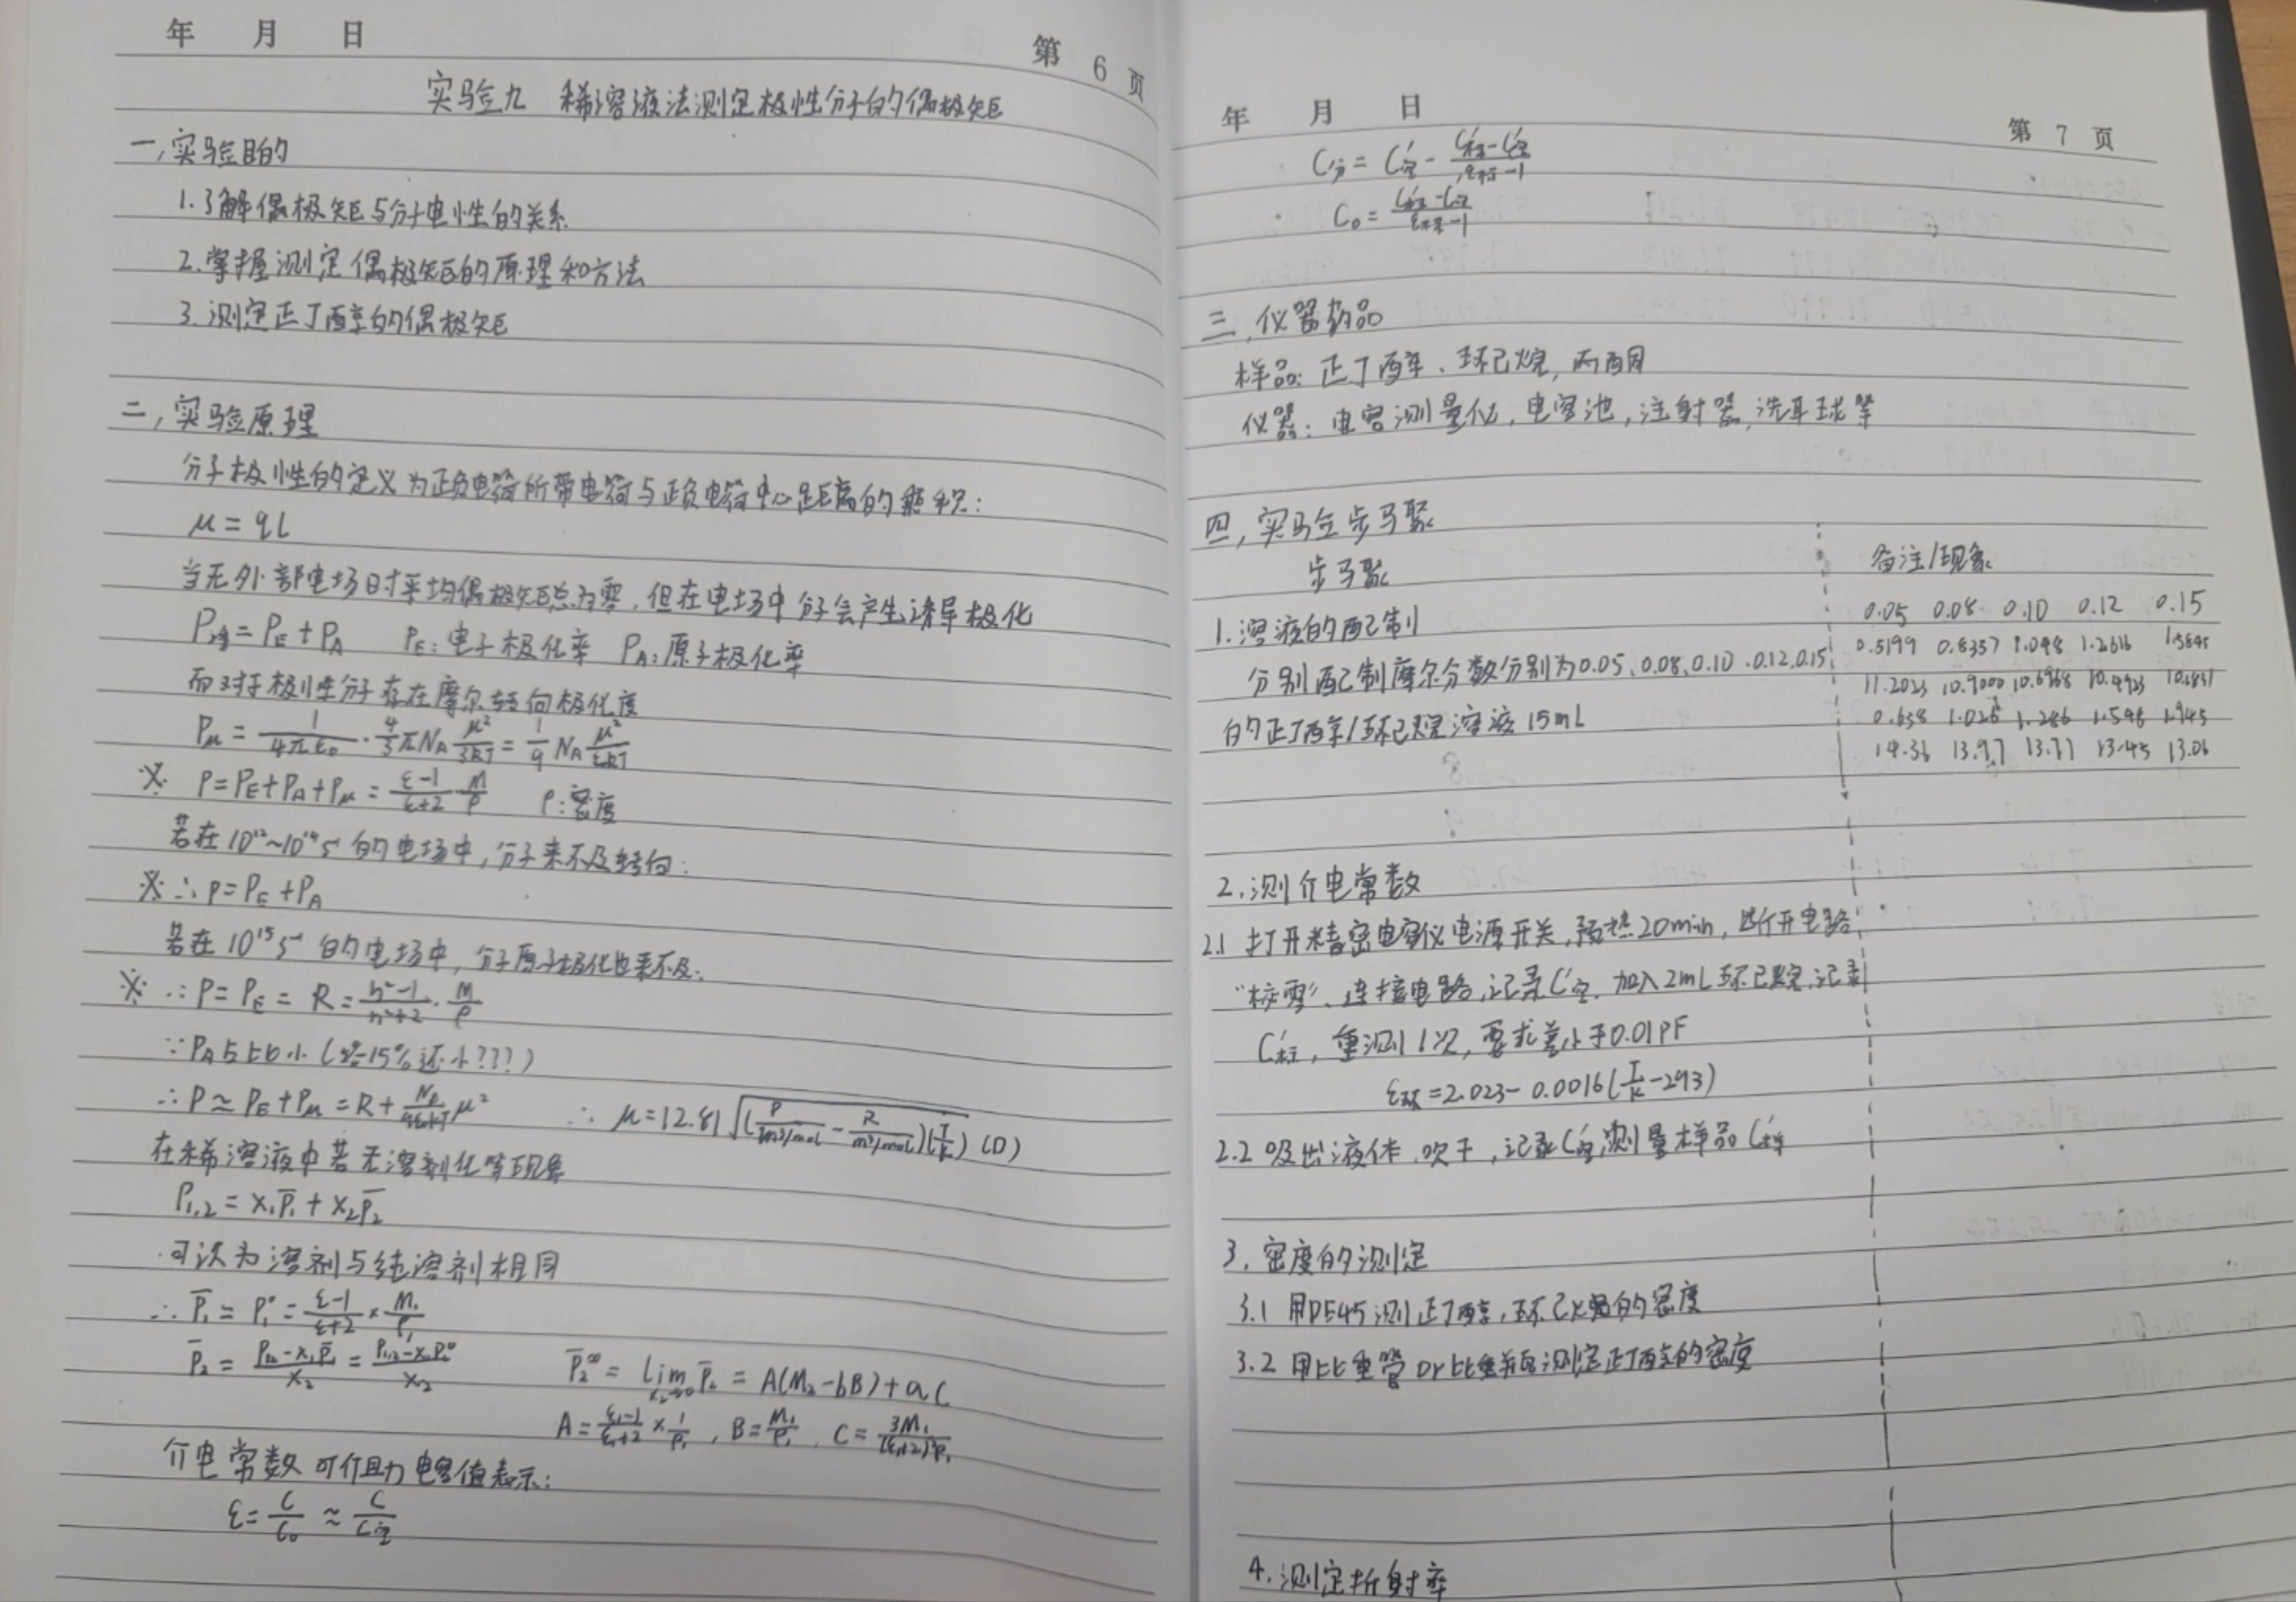
\includegraphics[width=1.0\textwidth]{1.png}
			\bicaption{实验预习报告的实验原理部分}{The principle part of the experiment in the experiment preview report}
		\end{figure}


               
	\vbox{} % 设置空行
	     
    \section{实验部分}
    	\subsection{仪器和试剂}
    		仪器:\ \  PCM-1A 型精密电容测量仪,电容池,玻璃注射器,洗耳球,50 mL 磨口锥形瓶,滴
			管,吸量管,比重管,DE45 型数字密度计,烧杯 (200 mL 两个),电子天平,阿贝折射仪,
			循环水真空泵;\par
			试剂:\ \  正丁醇 (AR),环己烷 (AR),丙酮 (AR),乙醇 (AR),去离子水;\par
    	\par
    	 \subsection{实验内容}
			\subsubsection{配制溶液}
				分别配置摩尔分数分别为0.05、0.08、0.10、0.12、0.15的正丁醇-环己烷溶液15ml并装在密闭锥形瓶中备用。称量过程中用电子天平准确称出各组分的质量,并计算摩尔分数,相应的数据被记录在\textbf{表1}中。
			\subsubsection{测量介电常数}
				打开精密电容仪开关,预热至少20min。断开电路,并校零。保证电容池内干燥后,测量该电容池以空气为介质的电容。
				取下电容池盖,像样品池中加满环己烷,并盖好电容池盖,读取此时的电容值。取下电容池盖,吸出其中的液体,并吹干。再次测量空气的电容值,要求两次测量的数据差值小于$0.01\ \rm{pF}$。 \par
				重复以上步骤测量样品的电容,用精密电容测量仪测量$5$个不同浓度的正丁醇溶液对应的电容值,直至相邻两次测定数据差不大于$0.01\ \ {\rm pF}$,记录数据。 \par
				
			\subsubsection{练习比重瓶测量密度}
				先称取空瓶的质量,随后将待测液体灌入瓶中,放入塞子,用滤纸擦干表面,盖上毛细管套,称取质量。以水为基准测量正丁醇。
				
			\subsubsection{密度的测定}
			用注射器吸取 \~{} 7\ mL\ 环己烷,向$\rm{DE45}$型数字密度计样品池中注入 \~{} \ 5\ mL\ 环己烷,排出气泡,按下“MEASURE”键测量环己烷密度;记录读数后再向样品池中注入 \~{}\ 1\ mL\ 环己烷,重复测量过程,共进行 3 次密度测量。测量完毕后排空样品池,长按“PUMP”键吹气除去样品池中剩余溶液。用同样的方法测定其余 5 种溶液及正丁醇的密度。
		\par	
			\subsubsection{折射率的测定}
				利用阿贝折射仪测定正丁醇的折射率。

				
    	
	\vbox{}
	 \section{数据与结果}
 		\subsection{实验数据记录及处理}
 			\subsubsection{溶液的配制及$X_{BuOH}$的计算}
				在溶液配置过程中,电子天平分别记录了锥形瓶的空重$\rm{m_{0}}$、加入环己烷后的质量$\rm{m_{1}}$以及总重$\rm{m_{2}}$ 。为了计算实际配置正丁醇-环己烷溶液的质量分数$X_{BuOH}$,需知道溶液中每个组分的质量。
				$$m_{BuOH}=\rm{m_{1}}-\rm{m_{0}}$$
				$$m_{Cy}=\rm{m_{2}}-\rm{m_{1}}$$
				最终溶液的$X_{BuOH}$可由公式\textbf{(1)}计算得到:\par
				$$X_{BuOH}= \frac{m_{BuOH}/M_{BuOH}}{m_{BuOH}/M_{BuOH}+m_{Cy}/M_{Cy}} \eqno(1)$$ \par
				其中$\rm{M_{BuOH}}$为正丁醇的摩尔质量,$\rm{M_{Cy}}$为环己烷的摩尔质量。质量数据以及$X_{BuOH}$的计算值在\textbf{表1}中列出:\par
				\begin{table}[!htbp]
					\arrayrulecolor{Maroon}
					\centering
					\zihao{5}
					\bicaption{称量质量数据以及$X_{BuOH}$的计算值}{Weigh the quality data and the calculate value of $X_{BuOH}$}
					\begin{tabular}{ccccccccc}
						\toprule
						编号 & $m_{0}/{\rm g}$ & $m_{1}/{\rm g}$ & $m_{2}/{\rm g}$ & $m_{\rm BuOH}/{\rm g}$ & $m_{\rm Cy}/{\rm g}$ & $\chi_{\rm BuOH}$ \\
						\midrule
						1 & 58.985 & 70.013 & 70.560 & 0.547 & 11.028 & 0.0533 \\
						2 & 58.985 & 71.179 & 71.990 & 0.822 & 10.701 & 0.0792 \\
						3 & 61.267 & 71.179 & 72.842 & 1.029 & 10.546 & 0.0997 \\
						4 & 57.492 & 67.785 & 69.009 & 1.224 & 10.293 & 0.1186 \\
						5 & 71.622 & 81.626 & 83.189 & 1.563 & 10.004 & 0.1507 \\
						\bottomrule
					\end{tabular}
				\end{table}

	 		\subsubsection{介电常数的测定以及计算}
			用精密电容测量仪测量环己烷以及溶液的电容,相关数据如\textbf{表2}所示。
			\begin{table}[h]
				\centering
				\zihao{5}
				\bicaption{各溶液电容值测定相关实验数据}{Correlative experimental data of determination of capacitance of each solution}
				\begin{tabular}{ccccccc}
					\toprule
					编号 & $C^{\prime}_{\rm E1}/{\rm pF}$ & $C^{\prime}_{\rm S1}/{\rm pF}$ & $C^{\prime}_{\rm E2}/{\rm pF}$ & $C^{\prime}_{\rm S2}/{\rm pF}$ & $\overline{C^{\prime}_{\rm E}}/{\rm pF}$ & $\overline{C^{\prime}_{\rm S}}/{\rm pF}$ \\
					\midrule
					Cy & 4.06 & 6.52 & 4.06 & 6.52 & 4.06 & 6.52 \\
					1  & 4.06 & 6.74 & 4.06 & 6.74 & 4.06 & 6.74 \\
					2  & 4.06 & 6.88 & 4.06 & 6.88 & 4.06 & 6.88 \\
					3  & 4.06 & 7.02 & 4.06 & 7.02 & 4.06 & 7.02 \\
					4  & 4.06 & 7.14 & 4.06 & 7.14 & 4.06 & 7.14 \\
					5  & 4.06 & 7.38 & 4.06 & 7.38 & 4.06 & 7.38 \\
					\bottomrule
				\end{tabular}
			\end{table}
			已知环己烷的介电常数$\varepsilon_{\rm Cy}$与温度$T$的关系为:
			$$
			\varepsilon_{\rm Cy}=2.023-0.0016\ \ (\frac{T}{\rm K}-293) \eqno(2)
			$$
			其中$T$为实验室温度,笔者实验时实验室温度位于$297.25\ \rm{K}$到$300.75\ \rm{K}$之间,考虑到测量电容时温度在$299.95\ \rm{K}$附近,代入$T=299.95\ \rm{K}$,可得$\varepsilon_{\rm Cy}=2.012$。 \par
			电容器的电容$C_{0}$可由公式\textbf{(3)}求算:
			$$
			C_{0}=\frac{C^{\prime}_{\rm Cy}-C^{\prime}_{\rm E}}{\varepsilon_{\rm Cy}-1}=\frac{6.52-4.06}{2.012-1}{\rm pF}= 2.431\eqno(3)
			$$
			分布电容$C_{\rm D}$(D即Distribution)可由公式\textbf{(4)}求算:
			$$
			C_{\rm D}=C^{\prime}_{\rm E}-C_{0}=4.06\ \ {\rm pF}-2.43\ \ {\rm pF}= 1.63\ \ {\rm pF} \eqno(4)
			$$
			可以近似认为分布电容$C_{\rm D}$为常数,在实验过程中保持不变,则样品的介电常数$\varepsilon_{\rm S}$可由公式\textbf{(5)}求算:
			$$
			\varepsilon_{\rm S}=\frac{C_{\rm S}}{C_{0}} \eqno(5)
			$$
			其中
			$$
			C_{\rm S}=C^{\prime}_{\rm S}-C_{\rm D}
			$$
			各溶液的介电常数$\varepsilon_{\rm S}$计算结果如\textbf{表3}所示:
			\begin{table}[h]
				\centering
				\zihao{5}
				\bicaption{各溶液介电常数$\varepsilon_{\rm S}$计算数据}{Calculation data of dielectric constant $\varepsilon_{\rm S}$ of each solution}
				\begin{tabular}{ccccc}
					\toprule
					编号 & $\chi_{\rm BuOH}$ & $C_{0}/{\rm pF}$ & $C_{\rm S}/{\rm pF}$ & $\varepsilon_{\rm S}$ \\
					\midrule
					1 & 0.0533 & 2.43 & 5.11 & 2.103 \\
					2 & 0.0792 & 2.43 & 5.25 & 2.160 \\
					3 & 0.0997 & 2.43 & 5.39 & 2.218 \\
					4 & 0.1186 & 2.43 & 5.51 & 2.267 \\
					5 & 0.1507 & 2.43 & 5.75 & 2.366 \\
					\bottomrule
				\end{tabular}
			\end{table}
			\par
			根据\textbf{表3}数据,作出$\varepsilon_{\rm S}-\chi_{\rm BuOH}$关系的散点图,并进行线性拟合,作出拟合直线,如\textbf{图2}所示。
			\begin{figure}[h]
				\centering
				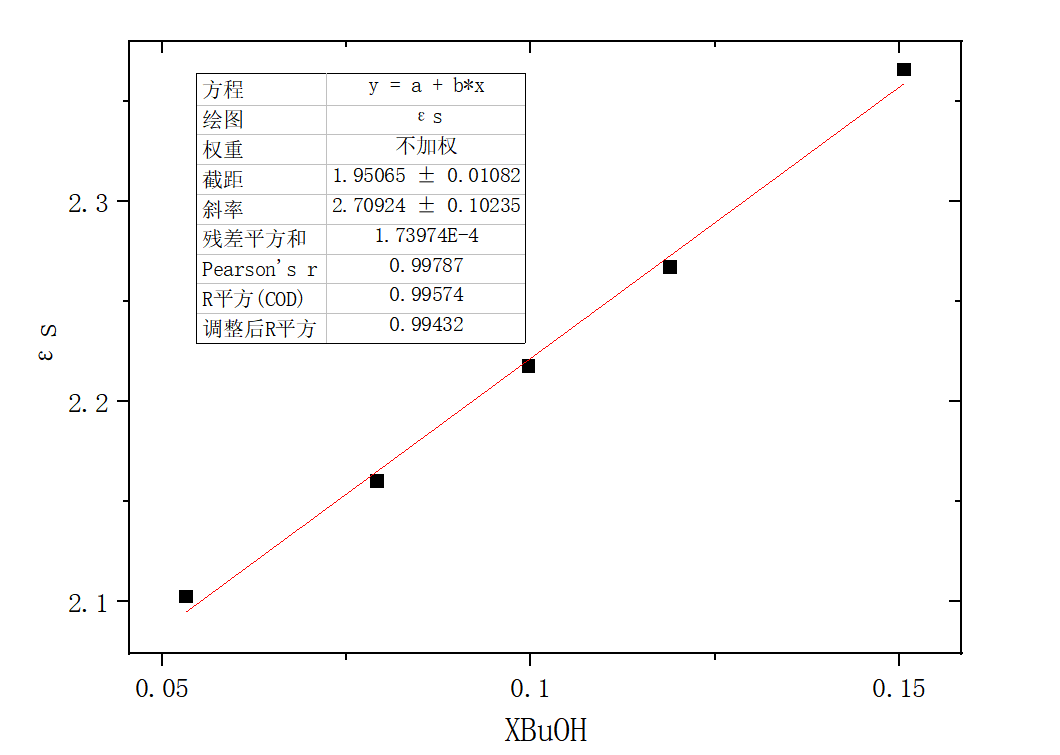
\includegraphics[width=0.8\textwidth]{2.png}
				\bicaption{$\varepsilon_{\rm S}-\chi_{\rm BuOH}$关系图及线性拟合}{$\varepsilon_{\rm S}-\chi_{\rm BuOH}$ diagram and linear fit}
			\end{figure}
			\par
			拟合直线的方程为
			$$
			\varepsilon_{\rm S}=(2.71\pm 0.1)\chi_{\rm BuOH}+(1.95\pm 0.01),\  \ R=0.9979
			$$
			故直线截距
			$$\varepsilon_{1}=1.95\pm 0.01$$
			直线斜率
			$$a=2.71\pm 0.1$$
			\par
	 		\subsubsection{密度的测量}
			练习使用比重瓶测定液体密度,先称取空瓶的质量,随后将待测液体灌入瓶中,放入塞子,用滤纸擦干表面,盖上毛细管套,称取质量。相关数据如\textbf{表4}所示,其中$M_{1}$、$M_{2}$为加入去离子水后比重瓶质量的两次测量结果,$M_{\rm BuOH,1}$和$M_{\rm BuOH,2}$为加入$\rm BuOH$后比重瓶质量的测量结果、$M_{0}$为空比重瓶质量的测量结果。\par
			\begin{table}[h]
				\centering
				\zihao{5}
				\bicaption{使用比重管测定液体密度相关实验数据}{Correlative data of determination of liquid density using pycnometer}
				\begin{tabular}{ccccc}
					\toprule
					$M_{1}/{\rm g}$ & $M_{2}/{\rm g}$ & $M_{\rm BuOH,1}/{\rm g}$ & $M_{\rm BuOH,2}/{\rm g}$ & $M_{0}/{\rm g}$ \\
					\midrule
					26.605 & 26.606 & 25.653 & 25.654 & 21.687 \\
					\bottomrule
				\end{tabular}
			\end{table}
			故两次测量时水的质量为:
			$$m_{1}=M_{1}-M_{0}=4.918\ \ {\rm g}$$
			$$m_{2}=M_{2}-M_{0}=4.919\ \ {\rm g}$$
			水的质量的平均值$$m=\frac{m_{1}+m_{2}}{2}=4.918\ \ {\rm g}$$
			故两次测量时正丁醇的质量为:
			$$m_{3}=M_{\rm BuOH,1}-M_{0}=3.966\ \ {\rm g}$$
			$$m_{4}=M_{\rm BuOH,2}-M_{0}=3.967\ \ {\rm g}$$
			正丁醇的质量的平均值:$$m_{BuOH}=\frac{m_{3}+m_{4}}{2}=3.966\ \ {\rm g}$$
			查手册知室温\citealp{dean1992lange}$T=26.1\ \ {\rm ^{\circ}C}$下水的密度$\rho=0.99676\ \ {\rm g\cdot mL^{-1}}$,故计算正丁醇的密度:
			$$
			\rho_{\rm BuOH}=\frac{m_{\rm BuOH}}{m}\rho=\frac{3.967\times 0.99676}{4.918}=0.80401\ \ {\rm g\cdot mL^{-1}}
			$$
			\vbox{} % 设置空行
			用DE45型数字密度计准确测定各溶液的密度,计算溶液密度平行测定值的平均值$\overline{\rho}$,结果如\textbf{表5}所示。
			\begin{table}[h]
				\centering
				\zihao{5}
				\bicaption{各溶液密度测定相关实验数据}{Correlative experimental data of determination of density of each solution}
				\begin{tabular}{ccccc}
					\toprule
					编号 & $\rho_{1}/{\rm g\cdot mL^{-1}}$ & $\rho_{2}/{\rm g\cdot mL^{-1}}$ & $\rho_{3}/{\rm g\cdot mL^{-1}}$ & $\overline{\rho}/{\rm g\cdot mL^{-1}}$ \\
					\midrule
					Cy   & 0.77384 & 0.77383 & 0.77384 & 0.77384 \\
					1    & 0.77432 & 0.77427 & 0.77432 & 0.77430 \\
					2    & 0.77459 & 0.77458 & 0.77458 & 0.77458 \\
					3    & 0.77492 & 0.77493 & 0.77493 & 0.77493 \\
					4    & 0.77527 & 0.77527 & 0.77527 & 0.77527 \\
					5    & 0.77587 & 0.77587 & 0.77587 & 0.77587 \\
					BuOH & 0.80584 & 0.80584 & 0.80584 & 0.80584 \\
					\bottomrule
				\end{tabular}
			\end{table}
			根据\textbf{表1}及\textbf{表4}数据,作出$\overline{\rho}-\chi_{\rm BuOH}$关系的散点图,并进行线性拟合,作出拟合直线,如\textbf{图3}所示。\par
			\begin{figure}[h]
				\centering
				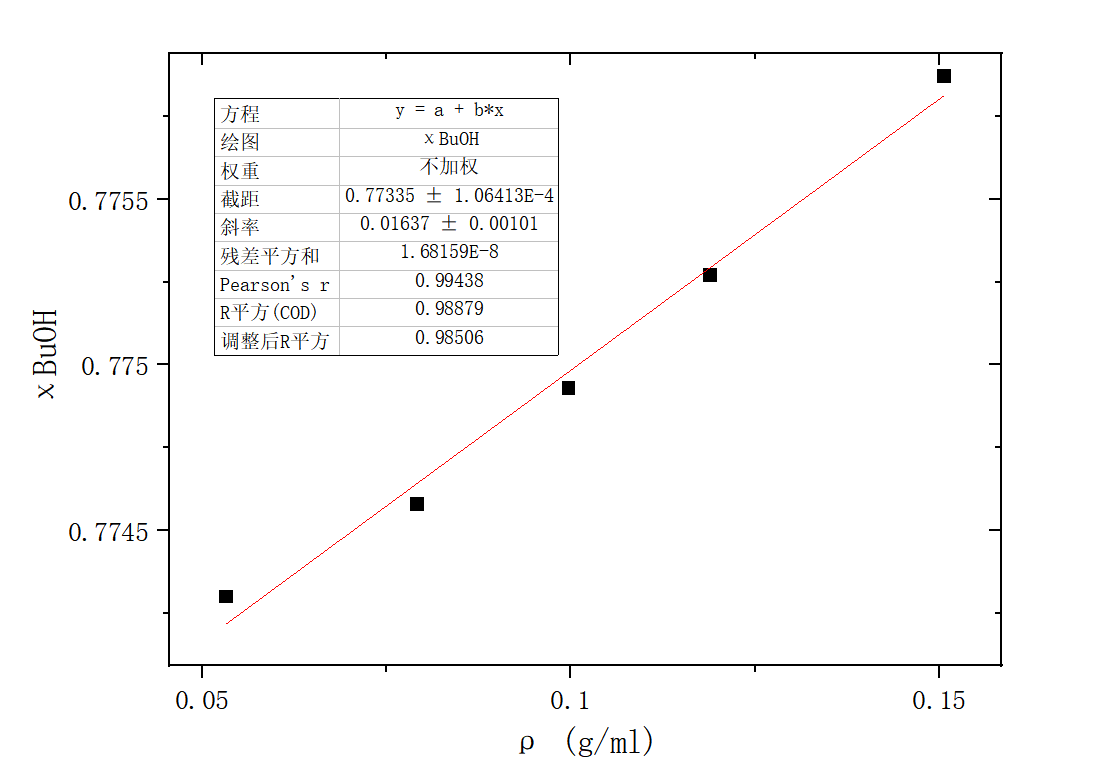
\includegraphics[width=0.8\textwidth]{3.png}
				\bicaption{$\overline{\rho}-\chi_{\rm BuOH}$关系图及线性拟合}{$\overline{\rho}-\chi_{\rm BuOH}$ diagram and linear fit}
			\end{figure}
			\par
			拟合直线的方程为
			$$
			\overline{\rho}=(0.0164\pm 0.001)\chi_{\rm BuOH}+(0.773\pm 0.0001),\  \ R=0.9888
			$$
			故直线截距
			$$\rho_{1}=0.773\pm 0.0001$$
			直线斜率
			$$b=0.0164\pm 0.001$$
			\par
			\subsubsection{折射率的测定和计算}
			用阿贝折射仪测定正丁醇在$297.25\ \rm{K}$下的折射率:
			$$
			n_{\rm BuOH}=1.3969
			$$
			正丁醇的折射度$R$可由公式\textbf{(6)}求算:
			$$
			R=\frac{n_{\rm BuOH}^{2}-1}{n_{\rm BuOH}^{2}+2}\times \frac{M_{\rm BuOH}}{\rho_{\rm BuOH}} \eqno(6)
			$$
			将$n_{\rm BuOH}$、$M_{\rm BuOH}$、$\rho_{\rm BuOH}$代入\textbf{(6)},可得正丁醇的折射度: \par
			$$
			R=\frac{1.3969^{2}-1}{1.3969^{2}+2}\times \frac{74.12\ \ {\rm g\cdot mol^{-1}}}{0.80584\ \ {\rm g\cdot mL^{-1}}}=22.145\ \ {\rm mL\cdot mol^{-1}}
			$$
		\vbox{} % 设置空行
		\subsection{计算与实验结果}
			\subsubsection{$\overline{P}^{\infty}_{2}$的计算}
			正丁醇的摩尔极化度$\overline{P}^{\infty}_{2}$可由公式\textbf{(7)}近似求算:
			$$
			\overline{P}^{\infty}_{2}=A(M_{2}-bB)+aC \eqno(7)
			$$
			其中,
			$$
			A=\frac{\varepsilon_{1}-1}{\varepsilon_{1}+2}\times \frac{1}{\rho_{1}}
			$$
			$$
			B=\frac{M_{1}}{\rho_{1}}
			$$
			$$
			C=\frac{3M_{1}}{(\varepsilon_{1}+2)^{2}\rho_{1}}
			$$
			由3.1 部分的数据处理可知$\varepsilon_{1}=1.95\pm 0.01$,$a=2.71\pm 0.1$,$\rho_{1}=(0.773\pm 0.0001)\ \ {\rm g\cdot mL^{-1}}$,$b=(0.0164\pm 0.001)\ \ {\rm g\cdot mL^{-1}}$、$M_{1}=84.16\ g\cdot mol^{-1} $、$M_{2}=74.12\ g\cdot mol^{-1} $,代入计算得:
			$$
			A=0.311\ \ {\rm mL\cdot g^{-1}}
			$$
			$$
			B=108.875\ \ {\rm mL\cdot mol^{-1}}
			$$
			$$
			C=20.93\ \ {\rm mL\cdot g^{-1}}
			$$
			$$
			\overline{P}^{\infty}_{2}= 79.22\ \ {\rm mL\cdot mol^{-1}}
			$$
			不确定度计算:
			$$
			\sigma_{A}=\sqrt{( \frac{3}{(\varepsilon_{1}+2)^{2}} \times  \frac{1}{\rho_{1}})^{2}\times \sigma^{2}_{\varepsilon_{1}}+(\frac{\varepsilon_{1}-1}{\varepsilon_{1}+2}\times \frac{1}{\rho_{1}})^{2}\sigma^{2}_{\rho_{1}}}=0.004\ \ {\rm mL\cdot mol^{-1}}
			$$
			$$
			\sigma_{B}=B\frac{\sigma_{\rho_{1}}}{\rho_{1}}=\frac{108.9\times 0.0001}{0.773}\ \ {\rm g\cdot mol^{-1}}=0.014\ \ {\rm  mL\cdot mol^{-1}}
			$$
			$$
			\sigma_{C}=C\sqrt{(\frac{\sigma_{\varepsilon_{1}}}{\varepsilon_{1}+2})^{2}+(\frac{\sigma_{\rho_{1}}}{\rho_{1}})^{2}}=20.93\times \sqrt{(\frac{0.01}{1.95+2})^{2}+(\frac{0.0001}{0.773})^{2}} \ \ {\rm mL\cdot mol^{-1}}=0.053\ \ {\rm mL\cdot mol^{-1}}
			$$ 
			故
			$$
			A=(0.307\pm 0.004)\ \ {\rm mL\cdot mol^{-1}}
			$$
			$$
			B=(108.169\pm 0.014)\ \ {\rm mL\cdot mol^{-1}}
			$$
			$$
			C=(21.1\pm 0.053)\ \ {\rm mL\cdot mol^{-1}}
			$$
			故$\overline{P}^{\infty}_{2}$的不确定度
			$$
			\sigma_{\overline{P}^{\infty}_{2}}=\sqrt{(M_{2}-bB)^{2} \sigma_{A}^{2}+A^{2} B^{2} \sigma_{b}^{2}+A^{2} b^{2} \sigma_{B}^{2}+C^{2} \sigma_{a}^{2}+a^{2} \sigma_{C}^{2}}=0.6\ \ {\rm mL\cdot mol^{-1}}
			$$
			故
			$$
			\overline{P}^{\infty}_{2}=(79.22\pm 0.6)\ \ {\rm mL\cdot mol^{-1}}
			$$
			\par
			\subsubsection{偶极矩的计算}
			正丁醇的偶极矩$\mu$可由公式\textbf{(7)}求算:
			$$
			\mu=12.81\sqrt{(\frac{\overline{P}^{\infty}_{2}}{\rm m^{3}\cdot mol^{-1}}-\frac{R}{\rm m^{3}\cdot mol^{-1}})(\frac{T}{K})}\ \ {\rm D} \eqno(7)
			$$
			由3.2.1知$\overline{P}^{\infty}_{2}=(79.22\pm 0.6) \ \ {\rm mL\cdot mol^{-1}}$,由3.1.3知$R=22.145\ \ {\rm mL\cdot mol^{-1}}$,$T=299.95\ \ {\rm K}$,代入公式计算得
			$$
			\mu=1.67\ \ {\rm D}
			$$
			考虑室温的波动,取$\sigma_{T}=1\ \ {\rm K}$,计算$\mu$的不确定度
			$$
			\sigma_{\mu}=\frac{12.81^{2}}{2} \sqrt{(\frac{T}{\mu})^{2} \sigma_{\overline{P}^{\infty}_{2}}^{2}+(\frac{\overline{P}^{\infty}_{2}-R}{\mu})^{2} \sigma_{T}^{2}}=0.01\ \ {\rm D}
			$$
			故
			$$
			\mu=(1.67\pm 0.01)\ \ {\rm D}
			$$
 	\section{讨论与结论}
		\subsubsection{实验误差}
		查阅\textit{CRC Handbook of Chemistry and Physics}\citealp{crc},知正丁醇偶极矩的文献值$\mu=(1.66\pm 0.03)\ \ {\rm D}$,相对误差:
			$$
			\xi=\frac{1.67-1.66}{1.66}\times 100\%=0.60\%
			$$
		可以注意到实验测得正丁醇偶极矩落在参考值范围内,与参考值很好地吻合,误差较小。
		\subsection{实验误差分析}
		尽管本次实验的误差较小,但依然存在一些步骤可能会引入误差:
		\begin{enumerate}
			\item 实验中所使用的精密电容仪出于电路接触等原因,其测量值在很大程度上会受到电容池和电容池盖摆放位置和方式的影响。经过笔者个人测试,同样的位置,电容池盖的摆放方式不同,测量值会相差$0.05\ \ {\rm pF}$左右,这已经足以产生较大误差。而实验中电容池盖的摆放方式无法控制,这必然会引入实验误差。
			\item 实验室中的温度并不恒定,测量折射度时的温度与测量电容时的温度相差约2摄氏度,这也会引入误差,同时实验室最初提供的吹风机,吹出的风明显高于室温,这也会导致电容的测量不准确。
			\item 在本实验中,大多数公式的推导都是基于理想稀溶液这一假设,仅仅在浓度比较低时才满足,然而在实验中,设计上的最大浓度已经达到了 0.15,这显然与稀溶液假设相悖。在测量密度的实验中,利用密度仪直接测量的密度$\overline{\rho}=0.77384\ {\rm g\cdot mL^{-1}}$而利用拟合得到的密度$\rho_{1}=0.77335\pm 0.0001$存在0.0005的偏差,虽然偏差较小但仍然存在,这也是稀溶液假设存在偏差的证明。
		\end{enumerate} \par
		造成偏差的主要原因推测是电容柜测量仪的位置与温度
 	 
 		\subsection{实验结论}
		 本实验通过稀溶液法测定正丁醇的偶极矩,通过测定不同浓度正丁醇-环己烷溶液密度、介电常数和正丁醇折射率,计算正丁醇摩尔极化度$\overline{P_{2}}^{\infty }=(a\pm b) \ ml\cdot mol^{-1} $。
		 利用阿贝折射仪测定正丁醇的折射率,进而求出其电子极化度也就是摩尔折射度$P_{E}=R=22.145 \ m^{3}\cdot mol^{-1}$ ,最终计算正丁醇偶极矩$\mu =1.67 \ D$,其与真实值相对偏差$\xi =0.60 \% $,造成偏差的主要原因推测是电容柜测量仪的位置与温度等。

\vbox{}  
%参考文献
\bibliographystyle{unsrt}
\bibliography{cite}
\end{document}